% This is "www2009-sample.tex" copied from "www2005-sample.tex" V1.2 January 26 2004
% This file should be compiled with V1.4 of "www2009-submission.class"
%
% This example file demonstrates the use of the 'www2009-submission.cls'
% V1.4 LaTeX2e document class file. It is for those submitting
% articles to the WWW'04 Conference WHO DO NOT WISH TO 
% STRICTLY ADHERE TO THE SIGS (PUBS-BOARD-ENDORSED) STYLE.
% The 'www2009-submission.cls' file will produce a similar-looking,
% albeit, 'tighter' paper resulting in, invariably, fewer pages.
%
% ----------------------------------------------------------------------------------------------------------------
% This .tex file (and associated .cls V1.4) produces:
%       1) NO Permission Statement
%       2) WWW'04-specific conference (location) information
%       3) The Copyright Line with ACM data
%       4) NO page numbers
%
% ---------------------------------------------------------------------------------------------------------------
% This .tex source is an example which *does* use
% the .bib file (from which the .bbl file % is produced).
% REMEMBER HOWEVER: After having produced the .bbl file,
% and prior to final submission, you *NEED* to 'insert'
% your .bbl file into your source .tex file so as to provide
% ONE 'self-contained' source file.
%
% ================= IF YOU HAVE QUESTIONS =======================
% Questions regarding the SIGS styles, SIGS policies and
% procedures, Conferences etc. should be sent to
% Julie Goetz (goetz@acm.org) or Adrienne Griscti (griscti@acm.org)
%
% Technical questions only to
% Gerald Murray (murray@acm.org)
% ===============================================================
%
% For tracking purposes - this is V1.2 - January 26 2004
\documentclass{www2009-submission}

\begin{document}
%
\title{DBpedia - A Linked Data Hub and Data Source for Web and Enterprise Applications}
%\subtitle{[Extended Abstract]
%\titlenote{A full version of this paper is available as
%\textit{Author's Guide to Preparing ACM SIG Proceedings Using
%\LaTeX$2_\epsilon$\ and BibTeX} at
%\texttt{www.acm.org/eaddress.htm}}}
%
% You need the command \numberofauthors to handle the "boxing"
% and alignment of the authors under the title, and to add
% a section for authors number 4 through n.
%
% Up to the first three authors are aligned under the title;
% use the \alignauthor commands below to handle those names
% and affiliations. Add names, affiliations, addresses for
% additional authors as the argument to \additionalauthors;
% these will be set for you without further effort on your
% part as the last section in the body of your article BEFORE
% References or any Appendices.

\numberofauthors{3}
%
% Put no more than the first THREE authors in the \author command

% NOTE: All authors should be on the first page. For instructions
% for more than 3 authors, see:
% http://www.acm.org/sigs/pubs/proceed/sigfaq.htm#a18

\author{
%
% The command \alignauthor (no curly braces needed) should
% precede each author name, affiliation/snail-mail address and
% e-mail address. Additionally, tag each line of
% affiliation/address with \affaddr, and tag the
%% e-mail address with \email.
\alignauthor Georgi Kobilarov\\
       \affaddr{Freie Universit�t Berlin}\\
       \affaddr{Garystr. 21}\\
       \affaddr{D-14195 Berlin, Germany}\\
       \email{georgi.kobilarov@fu-berlin.de}
\alignauthor Christian Bizer\\
       \affaddr{Freie Universit�t Berlin}\\
       \affaddr{Garystr. 21}\\
       \affaddr{D-14195 Berlin, Germany}\\
       \email{chris@bizer.de}
\and
\alignauthor S�ren Auer\\
       \affaddr{Universit�t Leipzig}\\
       \affaddr{Johannisgasse 26}\\
       \affaddr{D-04103 Leipzig, Germany}\\
       \email{auer@uni-leipzig.de}
\alignauthor Jens Lehmann\\
       \affaddr{Universit�t Leipzig}\\
       \affaddr{Johannisgasse 26}\\
       \affaddr{D-04103 Leipzig, Germany}\\
       \email{lehmann@informatik.uni-leipzig.de}
}
\date{27 March 2009}

\maketitle
\begin{abstract}
The DBpedia project has extracted a rich knowledge base from Wikipedia and serves this knowledge base as Linked Data on the Web. DBpedia's knowledge base currently provides 274 million pieces of information about 2.6 million concepts. As DBpedia covers a wide range of domains and has a high degree of conceptual overlap with various open-license datasets that are already available on the Web, an increasing number of data publishers has started to set data links from their data sources to DBpedia, making DBpedia one of the central interlinking hubs of the emerging Web of Data. This paper gives an overview about the DBpedia project and describes how application developers can make use of DBpedia knowledge within their applications.
\end{abstract}

% A category with only the three required fields
\category{H.4.m}{Information Systems}{Miscellaneous}

%\terms{Documentation, Standardization}

\keywords{Web of Data, Linked Data, Knowledge Extraction, Wikipedia, DBpedia}

\section{Introduction}
Knowledge bases are playing an increasingly important role in enhancing the intelligence of Web and enterprise search and in supporting information integration. Today, most knowledge bases cover only specific domains, are created by relatively small groups of knowledge engineers, and are very cost intensive to keep up-to-date as domains change. At the same time, Wikipedia has grown into one of the central knowledge sources of mankind, maintained by thousands of contributors. The DBpedia project~\cite{dbpedia} leverages this gigantic source of knowledge by extracting structured information from Wikipedia and by making this information accessible on the Web.

The DBpedia knowledge base currently describes more than 2.6 million things, including at least 213,000 persons, 328,000 places, 57,000 music albums, 36,000 films, 20,000 companies. The knowledge base consists of 274 million pieces of information (RDF triples). It features labels and short abstracts for these things in 15 different languages; 609,000 links to images and 3,150,000 links to external web pages; 4,878,100 external links into other RDF datasets. Entities are classified in 4 concept hierarchies: The manually build DBpedia ontology, the YAGO~\cite{YagoArticle} ontology, the UMBEL\footnote{http://umbel.org} ontology and a SKOS representation of the Wikipedia category system. 
The DBpedia knowledge base has several advantages over existing knowledge bases: It covers many domains, it represents real community agreement, it automatically evolves as Wikipedia changes, and it is truly multilingual.

This paper is structured as follows: We give an overview of the DBpedia extraction framework and describe how Web applications can access the DBpedia knowledge base. Afterwards, we describe three use cases of the DBpedia knowledge base and its concept identifiers: Knowledge source for web applications; interlinking hub to connect data sources, and vocabulary for annotating web documents.


\section{DBpedia Extraction Framework}

While Wikipedia articles consist mostly of free text, they also contain various types of structured information, such as infobox templates, categorisation information, images, geo coordinates, links to external Web pages and other Wikipedia articles, disambiguation information, redirects and cross-language links. The DBpedia extraction framework extracts these different kinds of information and turns them into RDF data. 

All entities in DBpedia are assigned a unique URI of the form \texttt{http://dbpedia.org/resource/\emph{Name}}, where \emph{Name} is taken from the URL of the source Wikipedia article, which has the form \texttt{http://en.wikipedia.org/wiki/\emph{Name}}.

The type of wiki contents that are most valuable for the DBpedia extraction are Wikipedia infoboxes. Infoboxes contain attribute value pairs and are used to display an article's most relevant facts as a table at the top right-hand side of the corresponding Wikipedia page. Wikipedia's infobox template system has evolved over time without central coordination. Therefore, there is a lack of uniformity of infoboxes. Different templates use different names for the same attribute (e.g. \verb|birthplace| and \verb|placeofbirth|). While the first version of our infobox extractor used a generic method to turn property value pairs into triples and hence struggled with the different names of attributes, our new mapping-based extractor aims to solve that problem by introducing a central DBpedia ontology and mappings between templates and the ontology.

This ontology was created by manually arranging the 350 most commonly used infobox templates within the English edition of Wikipedia into a subsumption hierarchy consisting of 170 classes and then mapping 2300 attributes from within these templates to 720 ontology properties. The property mappings define fine-grained rules on how to parse infobox values and define target datatypes, which help the parsers to process values.

\begin{figure}[h]
	
		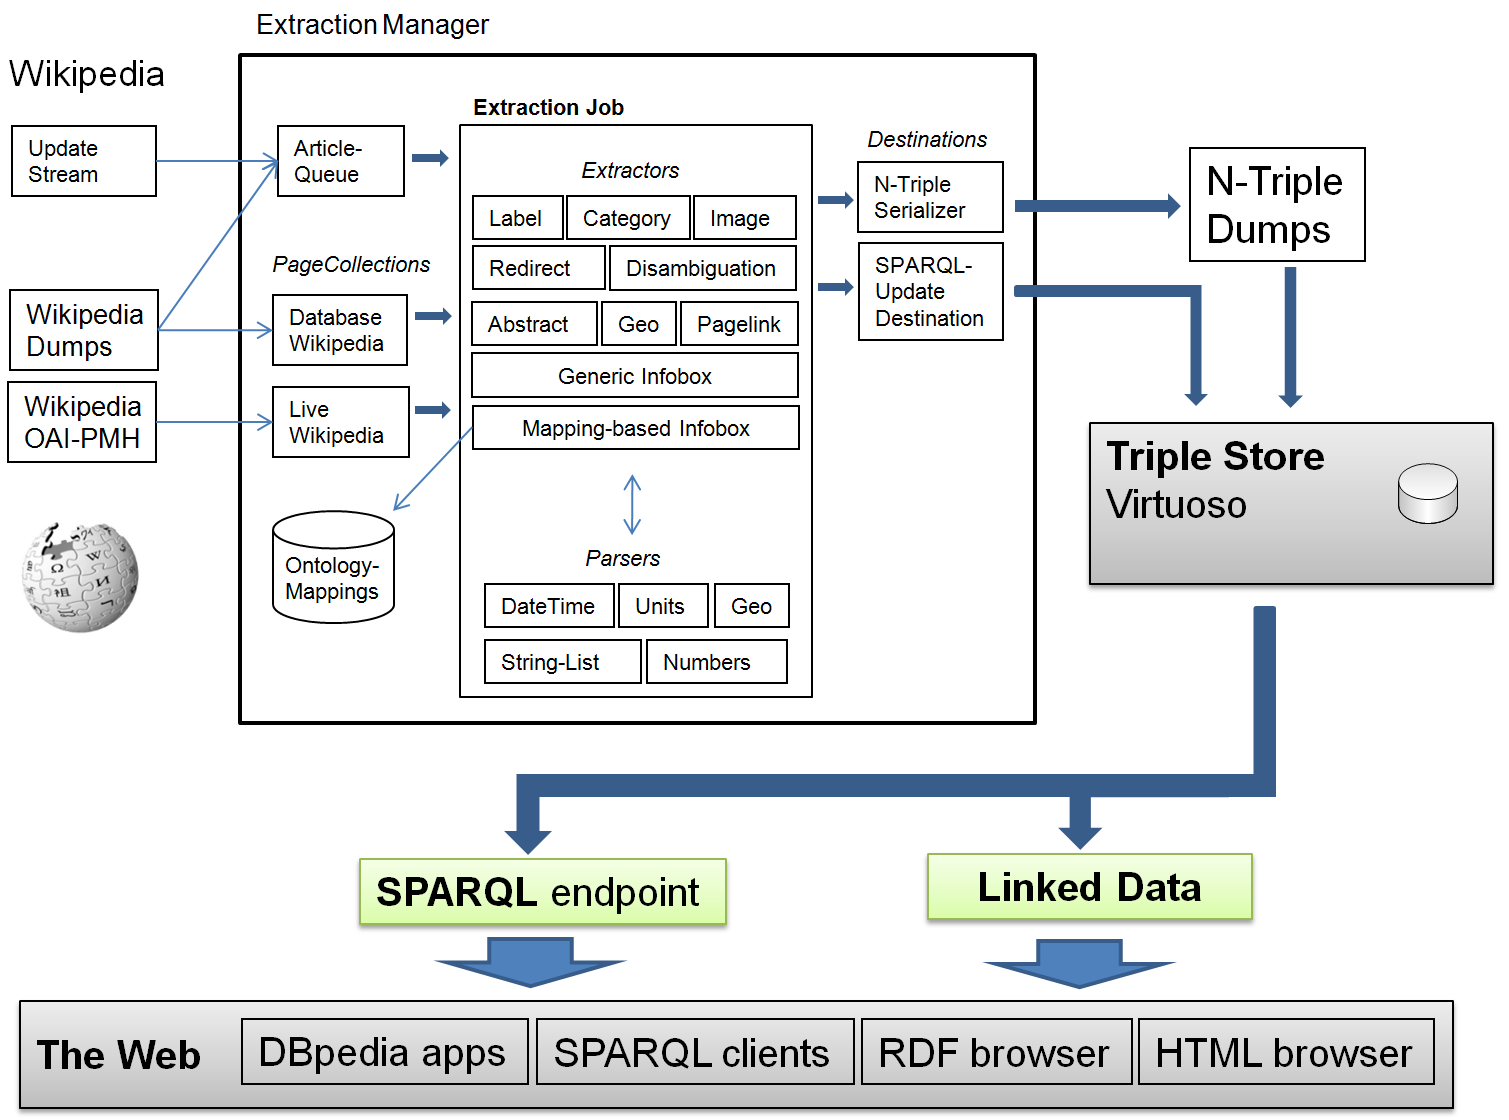
\includegraphics[width=0.48\textwidth]{architecture_extraction.png}
	\caption{Overview of DBpedia components.}
	\label{fig:architecture}
\end{figure}

Figure~\ref{fig:architecture} gives an overview of the open-source DBpedia extraction framework. The main components of the framework are: \emph{PageCollections} which are an abstraction of local or remote sources of Wikipedia articles, \emph{Destinations} that store or serialize extracted RDF triples, \emph{Extractors} which turn a specific type of wiki markup into triples, \emph{Parsers} which support the extractors by determining datatypes, conversion values between different units and splitting markup into lists. \emph{ExtractionJobs} group a page collection, extractions and a destination into a workflow. The core of the framework is the \emph{Extraction Manager} which manages the process of passing Wikipedia articles to the extractors and delivers their output to the destination. 

\section{Acessing DBpedia over the Web}

In order to fulfill the requirements of different client applications, we serve the DBpedia knowledge through four access mechanisms: 

\begin{description}
	\item [Linked Data.] DBpedia URIs be dereferenced over the Web according to the Linked Data principles~\cite{linkedData,linkedDataHowto}. DBpedia resource identifiers (such as \url{http://dbpedia.org/ resource/Berlin}) are set up to return (a) RDF descriptions when accessed by Semantic Web agents (such as data browsers or crawlers of Semantic Web search engines), and (b) a simple HTML view of the same information to traditional Web browsers. HTTP content negotiation is used to deliver the appropriate format.
 \item [SPARQL Endpoint.] We provide a SPARQL endpoint for querying the DBpedia knowledge base. Client applications can send queries over the SPARQL protocol to this endpoint at \url{http://dbpedia.org/sparql}.
 \item [RDF Dumps.] N-Triple serializations of the datasets are available for download at the DBpedia website at \newline	  \url{http://wiki.dbpedia.org/Downloads32}.
 \item [Lookup Index.] In order to make it easy for Linked Data publishers to find DBpedia resource URIs to link to, we provide a lookup service that proposes DBpedia URIs for a given label. The Web service is available at \url{http://lookup.dbpedia.org/api/search.asmx}.
\end{description}

\section{Use Cases}
This section describes three use cases of the DBpedia knowledge base and its concept identifiers.

\subsection{Data Source}

The DBpedia knowledge base is served on the Web under the terms of the GNU Free Documentation License. Application can therefore query the knowledge and use the query results, including labels and abstracts in 15 languages, for their purposes. Did you ever need a list and abstracts about 'Dutch cities over 200 meters altitude', 'Italian musicians from the 18th century', 'episodes of the HBO television show "The Sopranos"' or 'Software developed by an organisation founded in California by a person born in a European country in the 1960s' for your application? The DBpedia knowledge base can provide them for you. More sample SPARQL queries can be found on the DBpedia wiki at \verb|http://wiki.dbpedia.org|.

\begin{figure}[h]
    \centering
        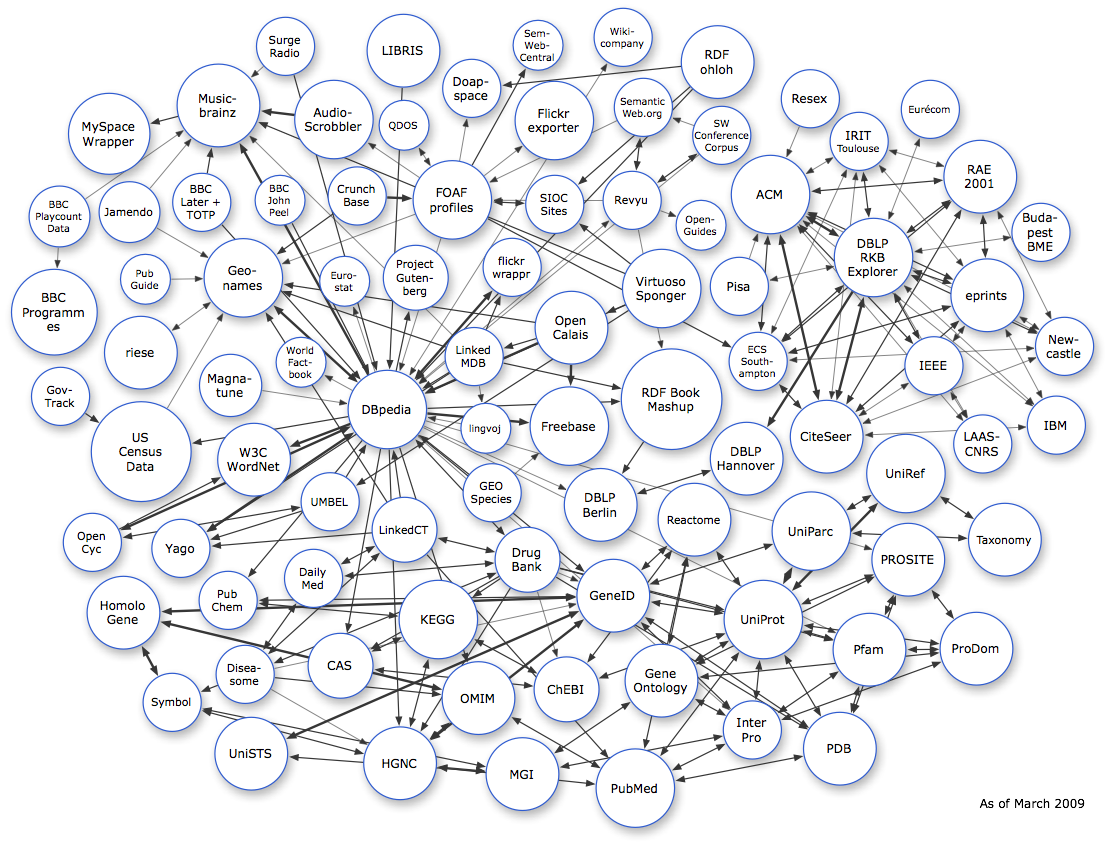
\includegraphics[width=0.48\textwidth]{lod-datasets_2009-03-05.png}
    \caption{The Linking Open Data Cloud}
    \label{fig:lod}
\end{figure}

\subsection{Interlinking Hub}
Linked Data~\cite{linkedData,linkedDataHowto} has become increasingly popular as a lightweight approach to publishing and connecting data on the Web. Over the last year, an increasing number of data publishers have started to set data links to DBpedia concepts, making DBpedia a central interlinking hub for the emerging Web of data. Currently, the Web of interlinked data sources around DBpedia provides around 4.5 billion pieces of information and covers domains such as geographic information, people, companies, films, music, genes, drugs, books, and scientific publications\footnote{http://esw.w3.org/topic/SweoIG/TaskForces/Community Projects/LinkingOpenData}.

A major advantage of using DBpedia as linking hub is that it contains semantic relations bridging different domains. This way specialized domain-specific datasets linked to DBpedia can be leveraged in cross domain (and cross dataset) queries. Figure~\ref{fig:lod} shows the cloud of interlinked data sources around DBpedia in the Linking Open Data Projekt. DBpedia itself links to external datasets with currently around 5 million outgoing RDF links, making it a good starting point for Semantic Web crawlers. Up to our knowledge, there are currently 21 external data sources that set RDF links to DBpedia. As link discovery engines such as \textit{Silk}~\cite{silkpaper} and \textit{ODDlinker}~\cite{oktei} make it increasingly easy to generate links between datasets, the data source network around DBpedia will hopefully keep on growing in the future.

Using DBpedia as interlinking hub is also a promising way to connect data sources within organizations. The BBC, for example, is using DBpedia as their main source of Linked Data identifiers and at the same time to link their data to the public Data Web~\cite{bbcdbpedia}. DBpedia identifiers are in the process of replacing other vocabularies, that were build by the BBC to  connect diverse data sources, as maintaining these vocabularies proved to be too expensive. 

\subsection{Content Annotation}
Annotating Web documents according to a global conceptual schema eases the discovery of content across Web sites. In addition to using DBpedia identifiers to interlink data sources on the Web, several projects have started to employ DBpedia URIs to annotate text documents. 
Named Entity Recognition (NER) services such as OpenCalais\footnote{http://www.opencalais.com}, MuddyBoots\footnote{http://www.muddy.it} or Zemanta\footnote{http://www.zemanta.com} use DBpedia URIs as identifiers for extracted entities or link their own identifiers to DBpedia URIs. The semantic bookmarking service Faviki\footnote{http://www.faviki.com} uses DBpedia identifiers for tagging Web pages similar to Delicious. 

A combination of named entity extraction and semantic content tagging can be found in the Content Ling Tool (see Figure~\ref{fig:ctt}) developed by the BBC. It allows BBC editors to annotated news articles~\cite{bbcdbpedia}. Here, the Muddy Boots service extracts named entities from the article text and identifies those with DBpedia URIs. In addition, editors can add annotations determining the topics of the articles using the auto-completion API of the DBpedia lookup service.

Semantic annotations allow the discovery of Web content that is related to a DBpedia entity and enable 3rd parties to enrich their content with data provided by DBpedia and interlinked data sources. Multiple documents annotated with the same URI of e.g. a musical artist can be related together and DBpedia can serve the structured background information about that artist with information such as her birthplace, the list of her albums or even movies containing one of her songs as part of their soundtracks. 

By using the same set of concept identifiers within textual documents and structured data, it therefore becomes possible to bridge between the classic document Web and the emerging Web of Data. 

\begin{figure}
    \centering
        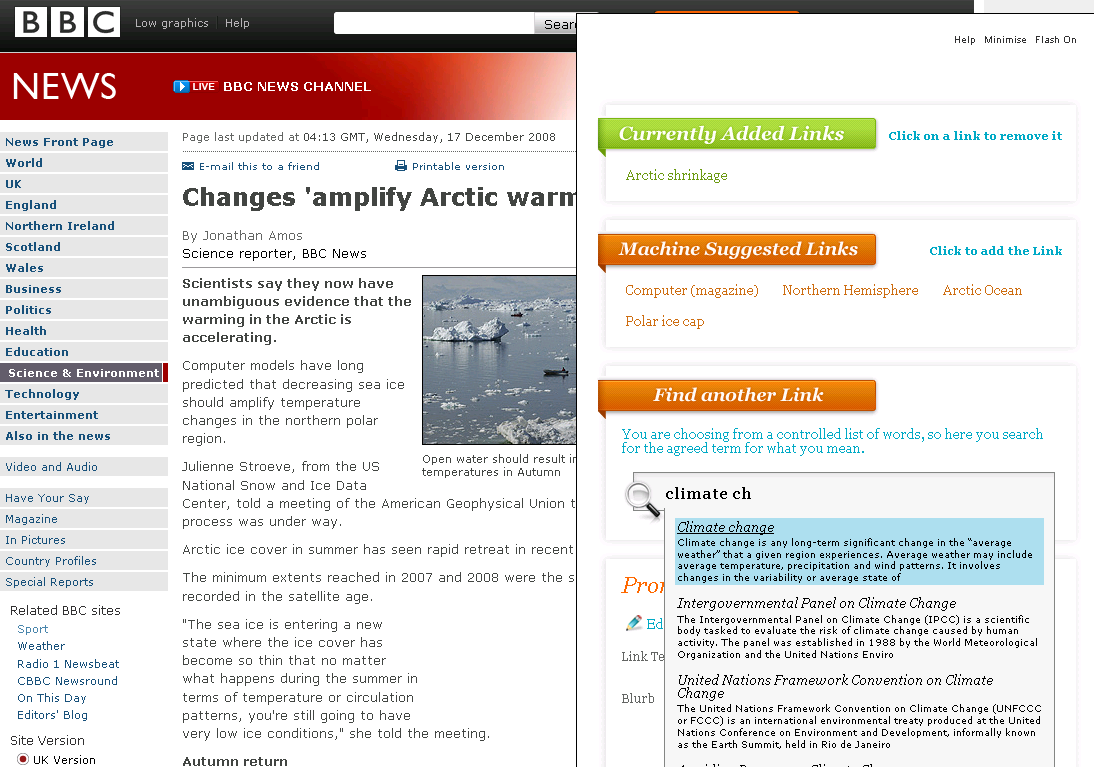
\includegraphics[width=0.48\textwidth]{CTT.PNG}
    \caption{Tagging BBC news articles with DBpedia URIs}
    \label{fig:ctt}
\end{figure}

\bibliographystyle{abbrv}
\bibliography{devtrack}  % sigproc.bib is the name of the Bibliography in this case
% You must have a proper ".bib" file
%  and remember to run:
% latex bibtex latex latex
% to resolve all references
%
% ACM needs 'a single self-contained file'!
%
%APPENDICES are optional
%\balancecolumns
\end{document}
